% Options for packages loaded elsewhere
\PassOptionsToPackage{unicode}{hyperref}
\PassOptionsToPackage{hyphens}{url}
%
\documentclass[
]{article}
\usepackage{amsmath,amssymb}
\usepackage{lmodern}
\usepackage{iftex}
\ifPDFTeX
  \usepackage[T1]{fontenc}
  \usepackage[utf8]{inputenc}
  \usepackage{textcomp} % provide euro and other symbols
\else % if luatex or xetex
  \usepackage{unicode-math}
  \defaultfontfeatures{Scale=MatchLowercase}
  \defaultfontfeatures[\rmfamily]{Ligatures=TeX,Scale=1}
\fi
% Use upquote if available, for straight quotes in verbatim environments
\IfFileExists{upquote.sty}{\usepackage{upquote}}{}
\IfFileExists{microtype.sty}{% use microtype if available
  \usepackage[]{microtype}
  \UseMicrotypeSet[protrusion]{basicmath} % disable protrusion for tt fonts
}{}
\makeatletter
\@ifundefined{KOMAClassName}{% if non-KOMA class
  \IfFileExists{parskip.sty}{%
    \usepackage{parskip}
  }{% else
    \setlength{\parindent}{0pt}
    \setlength{\parskip}{6pt plus 2pt minus 1pt}}
}{% if KOMA class
  \KOMAoptions{parskip=half}}
\makeatother
\usepackage{xcolor}
\IfFileExists{xurl.sty}{\usepackage{xurl}}{} % add URL line breaks if available
\IfFileExists{bookmark.sty}{\usepackage{bookmark}}{\usepackage{hyperref}}
\hypersetup{
  pdftitle={Notas probabilidad},
  hidelinks,
  pdfcreator={LaTeX via pandoc}}
\urlstyle{same} % disable monospaced font for URLs
\usepackage[margin=1in]{geometry}
\usepackage{color}
\usepackage{fancyvrb}
\newcommand{\VerbBar}{|}
\newcommand{\VERB}{\Verb[commandchars=\\\{\}]}
\DefineVerbatimEnvironment{Highlighting}{Verbatim}{commandchars=\\\{\}}
% Add ',fontsize=\small' for more characters per line
\usepackage{framed}
\definecolor{shadecolor}{RGB}{248,248,248}
\newenvironment{Shaded}{\begin{snugshade}}{\end{snugshade}}
\newcommand{\AlertTok}[1]{\textcolor[rgb]{0.94,0.16,0.16}{#1}}
\newcommand{\AnnotationTok}[1]{\textcolor[rgb]{0.56,0.35,0.01}{\textbf{\textit{#1}}}}
\newcommand{\AttributeTok}[1]{\textcolor[rgb]{0.77,0.63,0.00}{#1}}
\newcommand{\BaseNTok}[1]{\textcolor[rgb]{0.00,0.00,0.81}{#1}}
\newcommand{\BuiltInTok}[1]{#1}
\newcommand{\CharTok}[1]{\textcolor[rgb]{0.31,0.60,0.02}{#1}}
\newcommand{\CommentTok}[1]{\textcolor[rgb]{0.56,0.35,0.01}{\textit{#1}}}
\newcommand{\CommentVarTok}[1]{\textcolor[rgb]{0.56,0.35,0.01}{\textbf{\textit{#1}}}}
\newcommand{\ConstantTok}[1]{\textcolor[rgb]{0.00,0.00,0.00}{#1}}
\newcommand{\ControlFlowTok}[1]{\textcolor[rgb]{0.13,0.29,0.53}{\textbf{#1}}}
\newcommand{\DataTypeTok}[1]{\textcolor[rgb]{0.13,0.29,0.53}{#1}}
\newcommand{\DecValTok}[1]{\textcolor[rgb]{0.00,0.00,0.81}{#1}}
\newcommand{\DocumentationTok}[1]{\textcolor[rgb]{0.56,0.35,0.01}{\textbf{\textit{#1}}}}
\newcommand{\ErrorTok}[1]{\textcolor[rgb]{0.64,0.00,0.00}{\textbf{#1}}}
\newcommand{\ExtensionTok}[1]{#1}
\newcommand{\FloatTok}[1]{\textcolor[rgb]{0.00,0.00,0.81}{#1}}
\newcommand{\FunctionTok}[1]{\textcolor[rgb]{0.00,0.00,0.00}{#1}}
\newcommand{\ImportTok}[1]{#1}
\newcommand{\InformationTok}[1]{\textcolor[rgb]{0.56,0.35,0.01}{\textbf{\textit{#1}}}}
\newcommand{\KeywordTok}[1]{\textcolor[rgb]{0.13,0.29,0.53}{\textbf{#1}}}
\newcommand{\NormalTok}[1]{#1}
\newcommand{\OperatorTok}[1]{\textcolor[rgb]{0.81,0.36,0.00}{\textbf{#1}}}
\newcommand{\OtherTok}[1]{\textcolor[rgb]{0.56,0.35,0.01}{#1}}
\newcommand{\PreprocessorTok}[1]{\textcolor[rgb]{0.56,0.35,0.01}{\textit{#1}}}
\newcommand{\RegionMarkerTok}[1]{#1}
\newcommand{\SpecialCharTok}[1]{\textcolor[rgb]{0.00,0.00,0.00}{#1}}
\newcommand{\SpecialStringTok}[1]{\textcolor[rgb]{0.31,0.60,0.02}{#1}}
\newcommand{\StringTok}[1]{\textcolor[rgb]{0.31,0.60,0.02}{#1}}
\newcommand{\VariableTok}[1]{\textcolor[rgb]{0.00,0.00,0.00}{#1}}
\newcommand{\VerbatimStringTok}[1]{\textcolor[rgb]{0.31,0.60,0.02}{#1}}
\newcommand{\WarningTok}[1]{\textcolor[rgb]{0.56,0.35,0.01}{\textbf{\textit{#1}}}}
\usepackage{graphicx}
\makeatletter
\def\maxwidth{\ifdim\Gin@nat@width>\linewidth\linewidth\else\Gin@nat@width\fi}
\def\maxheight{\ifdim\Gin@nat@height>\textheight\textheight\else\Gin@nat@height\fi}
\makeatother
% Scale images if necessary, so that they will not overflow the page
% margins by default, and it is still possible to overwrite the defaults
% using explicit options in \includegraphics[width, height, ...]{}
\setkeys{Gin}{width=\maxwidth,height=\maxheight,keepaspectratio}
% Set default figure placement to htbp
\makeatletter
\def\fps@figure{htbp}
\makeatother
\setlength{\emergencystretch}{3em} % prevent overfull lines
\providecommand{\tightlist}{%
  \setlength{\itemsep}{0pt}\setlength{\parskip}{0pt}}
\setcounter{secnumdepth}{-\maxdimen} % remove section numbering
\ifLuaTeX
  \usepackage{selnolig}  % disable illegal ligatures
\fi

\title{Notas probabilidad}
\author{}
\date{\vspace{-2.5em}}

\begin{document}
\maketitle

\hypertarget{notas-probabilidad}{%
\subsection{Notas probabilidad}\label{notas-probabilidad}}

\hypertarget{definiciones-basicas}{%
\subsection{Definiciones basicas}\label{definiciones-basicas}}

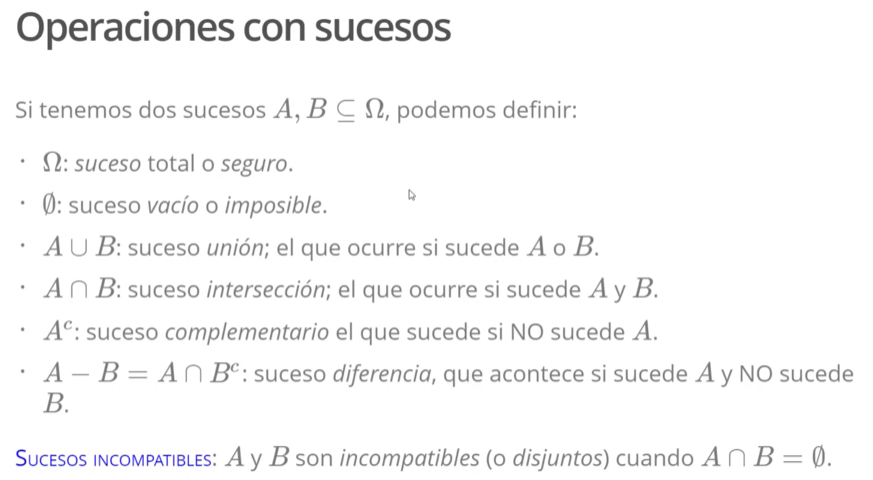
\includegraphics{images/paste-1AE55E3B.png}

\hypertarget{probabilidad-condicionada}{%
\subsection{Probabilidad condicionada}\label{probabilidad-condicionada}}

Ejemplos:

\begin{enumerate}
\def\labelenumi{\arabic{enumi}.}
\tightlist
\item
  Una empresa de telefonía tiene los siguientes clientes
\end{enumerate}

\[
\left.
\begin{array}{ll}
\text{75% 5G}\\
\text{80% Camera HD}
\end{array}
\right \}
\text{65% quiere los dos}
\]

Si elegimos una persona al azar de sus clientes, ¿Cuál es la
probabilidad que quieran al menos alguna de las dos cosas?

Definimos los dos sucesos:

\[
\begin{array}{ll}
\text{A = "El cliente quiere 5G"}\\
\text{B = "El cliente quiere camara HD"} 
\end{array}
\]

Conocemos las probabilidades:

\begin{Shaded}
\begin{Highlighting}[]
\NormalTok{p\_a }\OperatorTok{=} \FloatTok{.75}
\NormalTok{p\_b }\OperatorTok{=} \FloatTok{.8}
\NormalTok{p\_a\_i\_b }\OperatorTok{=} \FloatTok{.65}
\end{Highlighting}
\end{Shaded}

Por lo tanto queremos:

\[
P(\text{A}\cup\text{B}) = P(\text{A}) + P(\text{B}) - P(\text{A}\cap\text{B}) = 0.75 + 0.8 - 0.65 = 0.9
\]

\begin{Shaded}
\begin{Highlighting}[]
\NormalTok{p\_a }\OperatorTok{+}\NormalTok{ p\_b }\OperatorTok{{-}}\NormalTok{ p\_a\_i\_b}
\end{Highlighting}
\end{Shaded}

\begin{verbatim}
## 0.9
\end{verbatim}

El 90\% de nuestros clientes quieren como mínimo una de las
funcionalidades.

¿Cuál sería la probabilidad que una persona que quiere el 5G, cuál es la
probabilidad que quiera la cámara en HD, y una persona que quiere la
cámara quiera también el 5G?

Estas son probabilidades condicionadas:

\[
P(\text{B}\mid\text{A}) = \frac{P(\text{A}\cap\text{B})}{P(\text{A})} = \frac{0.65}{0.75} = .86
\\
P(\text{A}\mid\text{B}) = \frac{P(\text{A}\cap\text{B})}{P(\text{B})} = \frac{0.65}{0.8} = .81
\]

\begin{Shaded}
\begin{Highlighting}[]
\NormalTok{p\_a\_i\_b }\OperatorTok{/}\NormalTok{ p\_a}
\end{Highlighting}
\end{Shaded}

\begin{verbatim}
## 0.8666666666666667
\end{verbatim}

\begin{Shaded}
\begin{Highlighting}[]
\NormalTok{p\_a\_i\_b }\OperatorTok{/}\NormalTok{ p\_b}
\end{Highlighting}
\end{Shaded}

\begin{verbatim}
## 0.8125
\end{verbatim}

\hypertarget{fuxf3rmula-de-bayes}{%
\subsection{Fórmula de Bayes}\label{fuxf3rmula-de-bayes}}

Teorema de Bayes

Sean A y B dos sucesos. Si \(P(B) > 0\), entonces

\[
P(A \mid B) = \frac{P(A) * P(A \mid B)}{P(B)} = \frac{P(A) * P(B \mid A)}{P(A) * P(B \mid A) + P(A^c) * P(B \mid A^c)}
\]

\hypertarget{ejemplo}{%
\paragraph{Ejemplo:}\label{ejemplo}}

Uso de drogas en los deportes.

¿Qué tan bueno sería castigar a los atletas que han dado positivo en el
test de drogas?


\includegraphics[width=3.26042in,height=\textheight]{images/paste-1707571C.png}

Queremos estar seguros antes de culpar a una persona no culpable de que
ha tomado drogar.

Para ello lo primero que tenemos que hacer es definir los eventos que
corresponden al espacio muestral:

\begin{itemize}
\item
  \(D_{1}\) : usa drogas
\item
  \(D_{2}\) : no usa drogas
\item
  \(T_{1}\) : test de positivo
\item
  \(T_{2}\) : test da negativo
\end{itemize}

\[
\overline{C}
\]

\end{document}
